\documentclass[letterpaper, 12 pt, conference, onecolumn]{ieeeconf}  % Comment this line out if you need a4paper
%\documentclass[a4paper, 10pt, conference]{ieeeconf}      % Use this line for a4 paper

\IEEEoverridecommandlockouts                              % This command is only needed if 
                                                          % you want to use the \thanks command

\overrideIEEEmargins                                      % Needed to meet printer requirements.

% See the \addtolength command later in the file to balance the column lengths
% on the last page of the document

\usepackage[dvipdfmx]{graphicx}
\graphicspath{{figs/}}
\usepackage{amsmath}
\usepackage{amssymb}
\usepackage{algorithm}
\usepackage{algpseudocode}
\usepackage{times}
\usepackage[margin=1.1in]{geometry}
%
\newcommand{\figref}[1]{Fig.\ref{figure:#1}}
\newcommand{\tabref}[1]{Table \ref{table:#1}}
\newcommand{\argmax}{\operatornamewithlimits{argmax}}
\newcommand{\argmin}{\operatornamewithlimits{argmin}}

\title{\LARGE \bf
エージェントシステム レポート
}


\author{情報理工学系研究科創造情報学専攻, 情報システム工学研究室, \\
        48-166636, 和田健太郎, wada@jsk.imi.i.u-tokyo.ac.jp}

\begin{document}

\maketitle
\thispagestyle{empty}
\pagestyle{empty}

\section{研究テーマに関して}

私の研究テーマは多種物体の三次元認識とマニピュレーションで,
柔軟物や透明物体などを含んだ多様な物体の位置と状態を三次元的に理解し,
把持及び運搬を行う研究を行っている.

なぜこのような研究を行おうと考えたかというと,
多様なさらに複数の物体を同時に扱う必要のあるタスクは現在ロボットには困難であり,
それが可能となれば物流や生活支援など様々な応用先があると考えたからである.
多様な物体の中には,柔軟物のようにマニピュレーション中に変形する物や,
透明物体のようにセンシングが困難な物体も存在する.
さらに,それらが乱雑に配置されているような状況においては,
オクルージョンや影,物体同士の接触や結合など単一物体が整然とした環境で置かれている場合
と比べ様々な問題が発生する.

目指すところは,
少ない学習サンプルで多様な物体の位置を認識できるようにする``三次元認識''を実現し,
その認識結果にもとづいて物体をどうマニピュレーションするかという``動作計画''
を行い,複数物体マニピュレーションタスクを実現するということである.
現状では,三次元認識は少量のサンプル(6枚程度の物体画像)で実現可能なもの
となってきている.
しかし一方で,動作計画の部分はある環境を仮定した
ヒューリスティックなアルゴリズムとなっているため,
今後はより各環境状態に応じて動作計画を行う計画器を作成し,
環境が変化したとしても認識・動作可能なシステムの構築を実現したい.

エージェントシステムとの関係としては特に上で述べた動作計画の部分で,
現在人が与えている指令の部分を極力少なくし,
目的を与えるだけで動作を作成するような計画器(学習器)を作成したいと考えている.
私は現在,物体の倉庫内ピッキングタスクを複数物体マニピュレーションタスクとして
特に取り組んでいるが,物体が積み重なっている状況でどの物体を先にピッキングするかという
のが現在問題意識を持っていることの一つである.
物体の重なり具合には様々な組合せが存在し,単純に上から取っていけばよいというものではなく,
物体のZ座標の高さが最大でも,別の物体が斜めにその物体の上に重なっているというような
状況が存在する.
つまり物体群の画像を見た際に,各物体がどれほど他の物体によって隠れているかを判断し,
どれを先にPickingするかということを決定する機構が必要である.
さらにピッキングにおける目標物体が定められているような状況では,
多少その物体が隠れているような状況でも他の物体を押しのけて取ってしまう方が
タスクの全体時間が短くなりタスクも成功するため良い場合もある.
このようにどの物体を次の把持目標物体とするかという複数物体マニピュレーションの
ほんの一部の部分に関しても,タスクの目的からエージェントが学習する機構は応用可能であり,
授業で学んだことを今後活かしていきたいと考えている.  

\newpage

\section{シミュレータプログラムの応用}

OpenAI Gymを利用した強化学習として,
\figref{a}に示すような二つの環境で転ばないように
ゴールまでたどり着くロボットの学習を行った.
関節角をどう動かすかということがアクションとなっているので,
左だと股を開いた状態で動こうとするのが最初の局所解となるが,
学習がすすむと足を交差させるような不安定な状態を途中で取りながらも
速く走る動作を実現可能となった.
右の二本足のロボットでは,足ではなく頭と尻で歩行するような動作が得られ,
人が生成する場合には通常得られないような解が得られているということがわかる.
ここから,実際に現実世界のロボットなどに応用する場合には,
逆立ちは有効でないと考えられるため,
シミュレーションにおいては正確に条件を設定することが重要であると言える.

\begin{figure}[htbp]
  \centering
  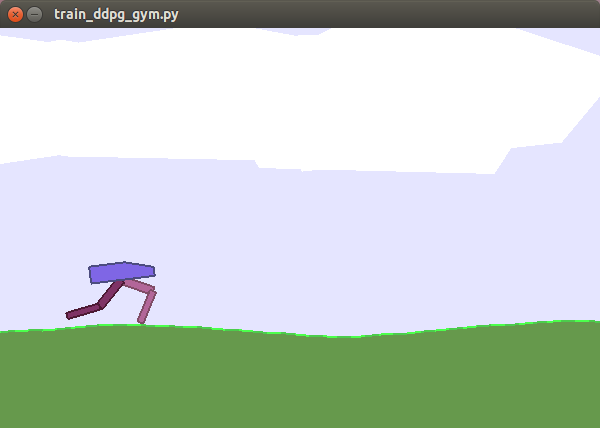
\includegraphics[width=0.5\columnwidth]{figs/a}
  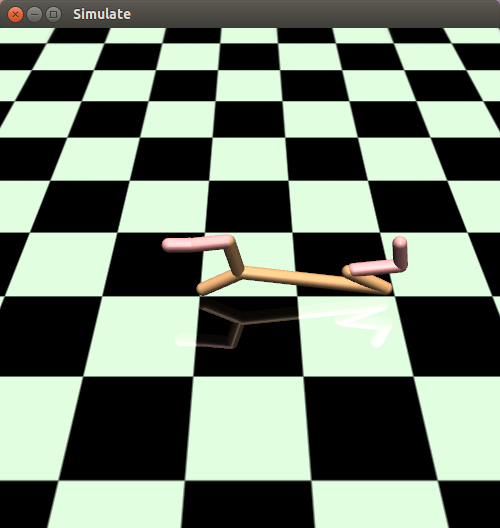
\includegraphics[width=0.34\columnwidth]{figs/b}
  \caption{Walking robot simulation.}
  \label{figure:a}
\end{figure}

\section{エージェントシステムにおける抽象化}

各システムの状態を抽象化し,その遷移条件を定義することで
全体のシステムを構築するステートマシンに関して考えたことを述べる.
実際にステートマシンをロボットシステムを構築するために応用してみて
(Amazon Robotics Challenge 2017にて),
各ステートを定義するとステート同士の遷移部分のみを
ハイパーパラメータとして設定できるということが分かった.
これはステートの遷移をパラメータで制御でき,
その組み合わせによって別のタスクを実現できる可能性があるという点で有用であると感じた.
これによって各ステートでの動作は個別に人や学習で作成し,
それらの遷移の部分をまた別の学習器によってタスクを成功するように学習させる
などということが可能である

\end{document}
